\documentclass[handout,aspectratio=169]{beamer}

\usepackage{amsmath, amsthm, amssymb, esint}
\usetheme{CambridgeUS}
\usecolortheme{seahorse}

\usepackage{graphicx}
\usepackage{float}

\title{MA109 Tutorial Session}
\subtitle{Week 3}
\author{Dhruv Arora}
\institute{Sophomore, Dept of CSE}
\date{\today}

\newtheorem{thm}{Theorem}
\newtheorem{cor}[thm]{Corollary}
\newtheorem{df}{Definition}
\newtheorem{qsn}{Question}

\newcommand{\bZ}{\mathbb{Z}}
\newcommand{\bN}{\mathbb{N}}
\newcommand{\bR}{\mathbb{R}}

\begin{document}

\begin{frame}[plain]
\titlepage
\end{frame}

\begin{frame}[plain]
\frametitle{What's New this Wednesday}
\tableofcontents
\end{frame}

\section{Tutorial Sheet 2}

\subsection{Q8. (ii) : Fitting a Function}

\begin{frame}
\frametitle{Q8. (ii)}
\pause
\begin{qsn}
Find a function $f:\bR\to\bR$ satisfying \pause
\begin{enumerate}
\item $f''(x)>0 \forall x \in \bR$ \pause
\item $f'(0)=1$ and $f'(1)=2$ \pause
\end{enumerate}
or otherwise show such a function cannot exist.
\end{qsn}
\end{frame}

\begin{frame}
\frametitle{Q8. (ii)}
A lot of functions satisfy the constraints.\\ \pause
You could fit a 2 degree polynomial with ease. \\ \pause 
I will fit an exponential function (because, strictly convex). \\[1mm] \pause
Consider $ae^{bx}$, with the given constraints, \\ [1mm] \pause
Verify that $\frac{2^x}{\ln 2}$ satisfies. \\[2mm] \pause
\small To be fair, you haven't defined $\ln$ or $e$ yet, so try to fit a quadratic!\\[2mm]
$x+\frac{x^2}{2}$ works!
\end{frame}

\subsection{Q8. (iii) : Fitting a Function}

\begin{frame}
\frametitle{Q8. (iii)}
\pause
\begin{qsn}
Find a function $f:\bR\to\bR$ satisfying \pause
\begin{enumerate}
\item $f''(x)\geq 0 \forall x \in \bR$ \pause
\item $f'(0)=1$ \ pause
\item $f(x)\leq 100 \forall x>0$ \pause
\end{enumerate}
or otherwise show such a function cannot exist.
\end{qsn}
\end{frame}

\begin{frame}
\frametitle{Q8. (iii)}
\textbf{Claim} : Such a function does not exist.
\pause
\begin{proof}[Proof. (by Contradiction)]
Assume such a function exists, let it be $f$. \\ \pause
$f(0)\leq 100$ (why?), so that $x_0 = 100-f(0) \geq 0$ \\ \pause
$f''(x)\geq 0$ on $\bR$ $\implies f'(x)$ is monotonically increasing on $\bR$ \\ \pause
$\forall x>0 \,\, f'(x)\geq f'(0) = 1 > 0 \implies f$ is strictly increasing on $(0,\infty)$ \\ 
Pick a $y>x_0$, now $\frac{f(y)-f(0)}{y-0} = f'(x)$ for some $x\in (0,y)$ \\
Note that $f(0)<f(y)\leq 100$ so $0 < f(y)-f(0) \leq 100-f(0)$ also, $y>100-f(0)$ \\
Thus, $f'(x)<1$ which contradicts the fact that $\forall x>0 \,\,f'(x)\geq 1$
\end{proof}
\end{frame}

\subsection{Q10. (i) : Sketching a Function}

\begin{frame}
\pause
\frametitle{Q10. (i)}
\begin{qsn}
Sketch the function defined on $\bR$ given by \pause
$$y=f(x)=2x^3+2x^2-2x-1$$ \pause
after identifying \pause
\begin{enumerate}
\item Intervals of increase/ decrease \pause
\item Intervalse of concavity and convexity \pause
\item Points of local maxima/minima \pause
\item Points of inflection \pause
\item Asymptotes 
\end{enumerate}
\end{qsn}
\end{frame}

\begin{frame}
\pause
\frametitle{Q10. (i)}
The function is polynomial, hence smooth! \\ \pause
The function does not have global extrema. (why?) \\ \pause
Get a reference point : $f(0) = -1$ (in general, try to get a few more) \\ \pause
$f'(x) = 6x^2+4x-2 = 2(3x-1)(x+1)$ is $\geq 0$ on $(-\infty,-1]\cup[1/3,\infty)$ and $\leq 0$ on $[-1,1/3]$ \\ \pause
These are intervals of increase and decrease \\ \pause
$\{-1,1/3\}$ are points of (possible) local extrema \\ \pause
$f''(x) = 12x+4$ which is $<0$ (concave) on $(-\infty,-1/3)$ and $>0$ (convex) on $(1/3,\infty)$ \\ \pause
So, indeed $-1$ is a point of local maxima, $1/3$ a point of local minima \\ \pause
Also, $-1/3 = [-1 + 1/3]/2$ (show this for any cubic) a point of inflection.
\end{frame}

\begin{frame}
\pause
\frametitle{Q10. (i)}
\begin{figure}[H]
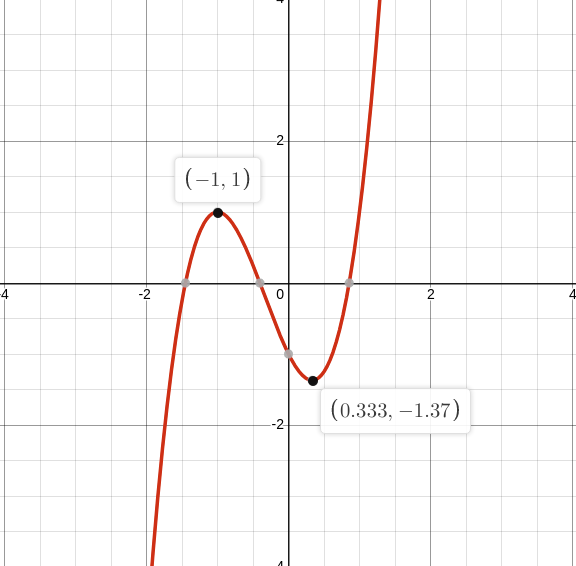
\includegraphics[scale=0.4]{plot.jpg}
\end{figure}
\end{frame}

\subsection{Q11 : Another Curve Fitting}

\begin{frame}
\frametitle{Q11}
\pause
\begin{qsn}
Sketch a continuous function $f:\bR\to\bR$ satisfying the following \\ \pause
\begin{enumerate}
\item $f(-2)=8, f(0)=4, f(2)=0$ \pause
\item $f'(x)>0$ for $|x|>2$ and $f'(x)<0$ for $|x|<2$ \pause
\item $f''(x)<0$ for $x<0$ and $f''(x)>0$ for $x>0$ 
\end{enumerate}
\end{qsn}
\end{frame}

\begin{frame}
\frametitle{Q11}
\textbf{Note} : I didn't mention $f'(2)=f'(-2)=0$ (why?) \\[1mm] \pause
We saw something similar just now. A cubic \textbf{might} have such properties!! \\[1mm] \pause
How to fit a cubic? Observe that now $f'(x) = c(x-2)(x+2)$, $c>0$ \\[1mm] \pause
Verify that this satisfies conditions (2) and (3) \\[1mm] \pause
Now the cubic will be of form $\frac{cx^3}{3}-4cx+d$ \\[1mm] \pause
$d=4$ and $c=3/4$ satisfy all constraints. \\[2mm] \pause
\begin{block}{Note}
This is not always guarenteed to work. Say, I change $f(0)=3$ instead. Can you still fit a cubic? Can you fit another function? Can you fit another polynomial?
\end{block}
\end{frame}

\begin{frame}
\pause
\frametitle{Q11}
\begin{figure}[H]
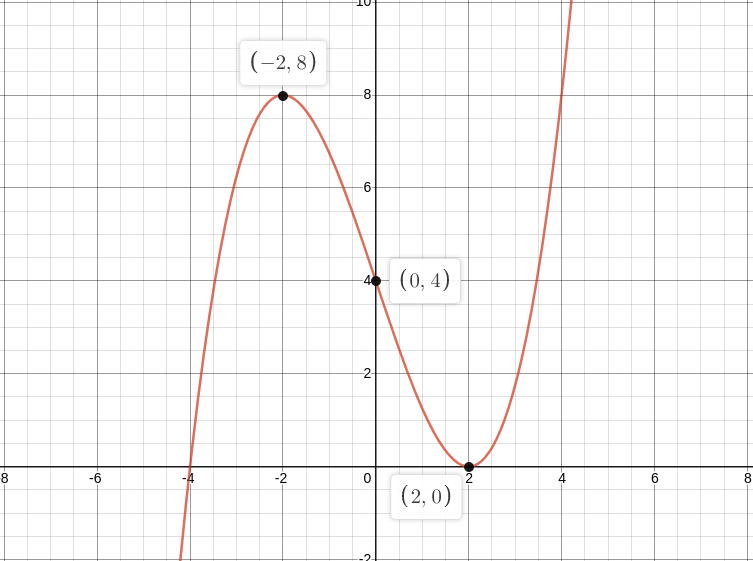
\includegraphics[scale=0.3]{plot2.jpg}
\end{figure}
\end{frame}

\section{Tutorial Sheet 3}

\subsection{Q1. (ii) : Taylor Series for $\tan ^{-1}$}

\begin{frame}
\frametitle{Q1. (ii)}
\pause
\begin{qsn}
Give the $n^{th}$ taylor polynomial and remainder of $\tan^{-1}(x)$ about $0$ when $|x|<1$
\end{qsn}
\end{frame}

\begin{frame}
\frametitle{Q1. (ii)}
\textbf{Claim} : The complete taylor expansion is $\tan^{-1}(x) = \sum\limits_{n=1}^\infty \frac{x^{2n-1}}{2n-1}$
\begin{proof}[Sketch. (Hacky)]
We find $f^{(n)}(x)$ and thus $f^{(n)}(0)$ \\ \pause
Observe $f'(x) = f^{(1)}(x) = \frac{1}{1+x^2} = \frac{1}{x-i}-\frac{1}{x+i}$ \\ \pause
Show by induction that $f^{(n)}(x) = \frac{(n-1)!(-1)^{n-1}}{2i} \left(\frac{1}{(x-i)^n} - \frac{1}{(x+i)^n}\right)$ \pause
$$f^{(n)}(0) = \begin{cases}
0 & n \text{ is even}\\
(n-1)!(-1)^{(n-1)/2} & n \text{ is odd}
\end{cases}$$
\end{proof}
\end{frame}

\begin{frame}
\frametitle{Q1. (ii)}
$P_\infty(x) = \sum\limits_{n=0}^{\infty} \frac{f^{(n)}(0)}{n!}x^n = \sum\limits_{n=1}^\infty \frac{x^{2n-1}}{2n-1}$ \\ \pause
To show convergence, you need to show $R_n(x) \to 0$ (try!) \\ \pause
A better method will be using integration like in Q5 \\ \pause
$$\tan^{-1}(x) = \int\limits_0^x \frac{1}{1+t^2}dt$$
Can you write a power series for $\frac{1}{1+x^2}$ with ease?
\end{frame}

\begin{frame}
\frametitle{The Rigorous Method}
Note that $\sum\limits_{n=0}^{\infty} (-t^2)^n = \frac{1}{1+t^2}$ for $|t|<1$ \\
This forms the power series expansion of $\frac{1}{1+t^2}$, so it can be integrated term by term \\
$$\tan^{-1}{x} = \int_{0}^{x} \frac{1}{1+t^2}dt = \int_{0}^{x} \sum\limits_{n=0}^{\infty} (-t^2)^n = \sum\limits_{n=0}^{\infty} (-1)^n \frac{x^{2n+1}}{2n+1}$$
This is the Taylor series expansion of $\tan^{-1}(x)$\footnote{I remember there was a doubt regarding this in class. The point is, if a function has a power series expansion about 0, it can be differentiated term by term as well. Can you use this to show that $a_n = f^{(n)}(0)/n!$?} \\
What is the remainder $R_n(x)$? There is no closed form solution. \\
Note that $R_{2m-1}(x) = R_{2m}(x) = \sum\limits_{n=m}^{\infty} (-1)^n \frac{x^{2n+1}}{2n+1}$ \\
You can write it as an integral!
\end{frame}


\subsection{Q2 : Taylor Series with an offset}

\begin{frame}
\frametitle{Q2}
\begin{qsn}
Write Taylor series of $f(x) = x^3-3x^2+3x-1$ about 1.
\end{qsn}
\pause
Taylor series about 1 will be \\ \pause
$$P_\infty(x) = \sum\limits_{n=0}^{\infty} \frac{f^{(n)}(1)}{n!} (x-1)^n$$ \pause
$f(x) = (x-1)^3$ hence $f^{(n)}(1) = 0 \forall n \neq 3$ \\ \pause
Verify that indeed $f(x) = P_\infty(x)$
\end{frame}

\subsection{Q4 : Convergence of $e^x$}

\begin{frame}
\frametitle{Q4}
\begin{qsn}
Show that the series $\sum_{k=0}^\infty \frac{x^k}{k!}$ converges.
\end{qsn}
\pause
\begin{proof}
Pick an $N>2|x|$, now for $n>N$, $\left|\frac{x^{n+1}}{(n+1)!}\right| \leq \frac{1}{2} \frac{|x|^n}{n!}$ \\ 
This can be seen as $|x/(n+1)| \leq |x/N| <1/2$, also, note $\frac{x^{n+1}}{(n+1)!} \leq \left|\frac{x^{n+1}}{(n+1)!}\right|$\\
Consider any $n>m>N$, then $\sum\limits_{k=n}^m \frac{x^k}{k!} \leq \sum\limits_{k=n}^m \frac{|x|^k}{k!} \leq \sum\limits_{k=N+1}^\infty\frac{|x|^k}{k!}$ \\ \pause
Using the inequality proved, show that $\sum\limits_{k=N+1}^\infty\frac{|x|^k}{k!}\leq \frac{|x|^N}{N!}$ (form a GP) \\ \pause
Since $\lim\limits_{n\to\infty} |x|^n/n! = 0$, we can find for any given $\epsilon>0$, a $M \in \bN$ such that $|x|^n/n! < \epsilon \forall n\geq M$ \\
Chose $N_0 = max\{N,M\}$. Show that this satisfies the cauchy definition.
\end{proof}
\end{frame}

\subsection{Q5 : $\int \frac{e^x}{x}$}

\begin{frame}
\frametitle{Q5}
\begin{qsn}
Write down a series for $\int \frac{e^x}{x}dx$
\end{qsn}
\pause
We write $\frac{e^x}{x} = \sum\limits_{n=0}^\infty \frac{x^{n-1}}{n!}$ \\ \pause
i.e. $\frac{e^x}{x} = \frac{1}{x}+\sum\limits_{n=1}^\infty \frac{x^{n-1}}{n!}$, so that \\
$\int \frac{e^x}{x} = \ln x + \sum\limits_{n=1}^\infty \frac{x^n}{n\cdot n!} + C$
\end{frame}

\end{document}